% !TeX encoding = UTF-8
% !TeX spellcheck = en_US
% !TeX root = ../00_first_presentation.tex
\begin{frame}{Robot Operating System (ROS)}
    \begin{itemize}
    \item The Robot Operating System (ROS) is a set of software libraries and tools that help you build robot applications. 
    \item Node: A process that uses ROS to communicate with other nodes.
    %\item Nodes get to know one another via roscore, that acts primarily as a server.
    \begin{figure}
    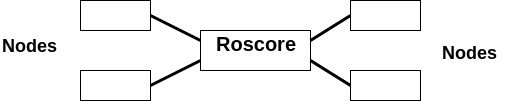
\includegraphics[scale=0.40]{roscore.jpg}
    \end{figure}
    \item Topic: Mechanism to send messages from a node to one or more nodes.
    \item Topic follows a publisher-subscriber design pattern.
    % where publisher is used to send message to topic, and subscriber get called when a message is published.
    \begin{figure}
    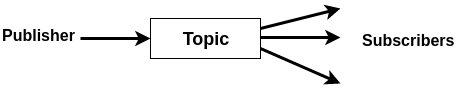
\includegraphics[scale=0.40]{topic.png}
    \end{figure}
    \end{itemize}
\end{frame}

\begin{frame}{continue...}
\begin{itemize}
\item Service: Mechanism for a node to send a request to another node  and receive a response in return.
\item Service follows a request-response design pattern.
\begin{figure}
    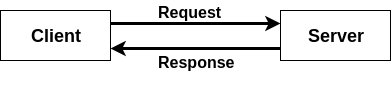
\includegraphics[scale=0.4]{service.png}
    \end{figure}
\item ROS supports two programming languages:
	\begin{itemize}
	\item C++
	\item Python
	\end{itemize}
\end{itemize}
\end{frame}